\chapter{Concept and Design}
\label{cha:conceptanddesign}

\section{General}

\section{Processes}

\subsection{Registration}

 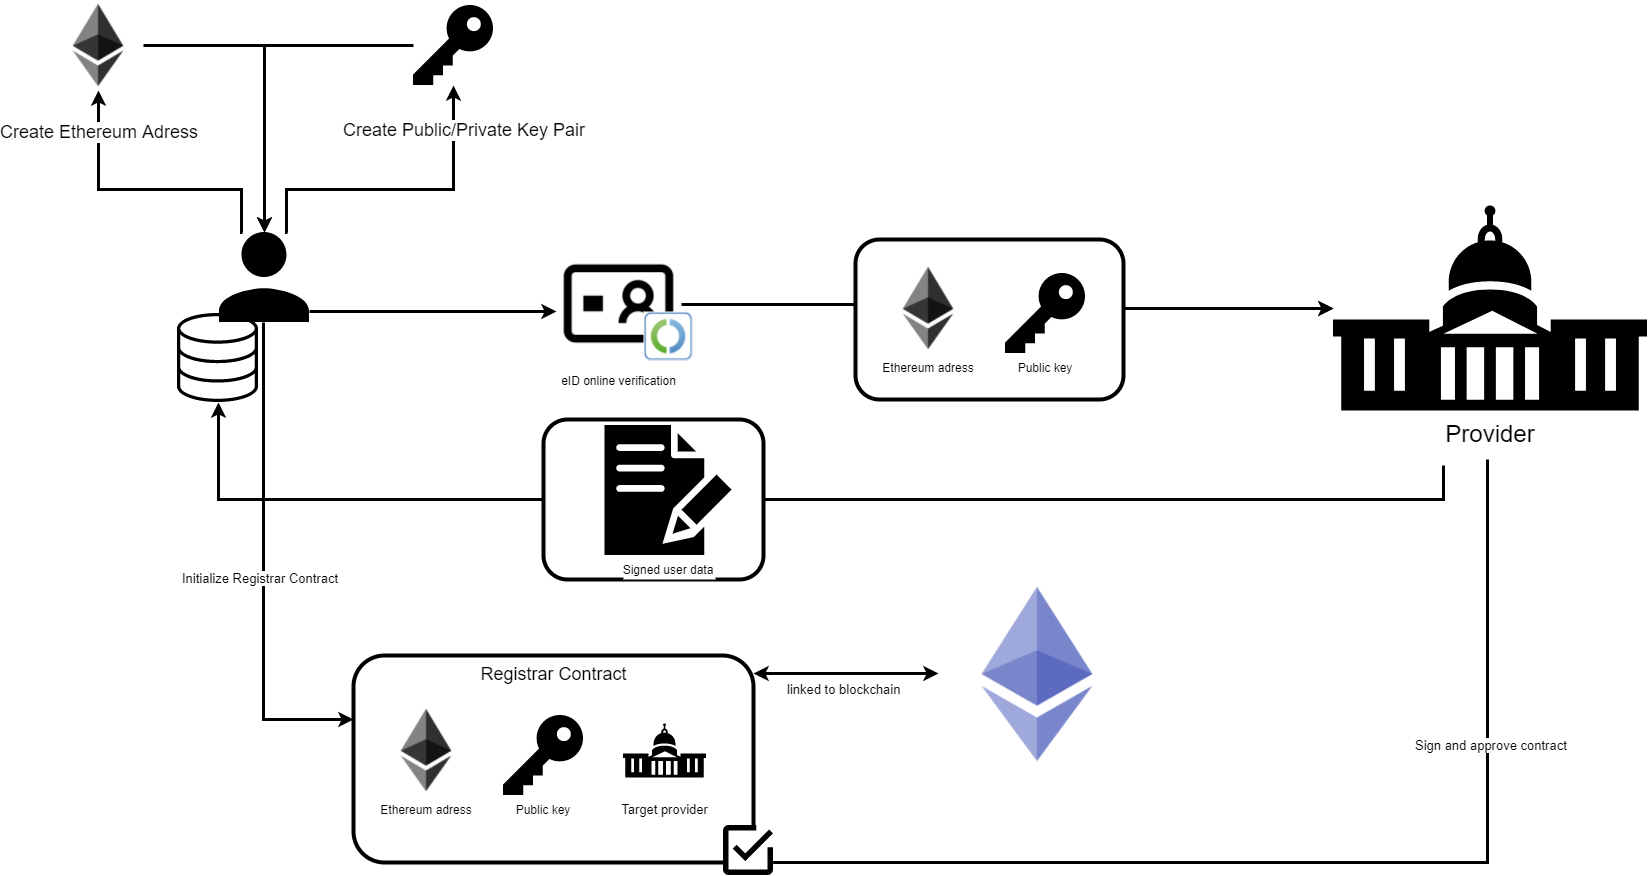
\includegraphics[width=\textwidth]{concept/registration.png}

\subsection{Permission Request}

 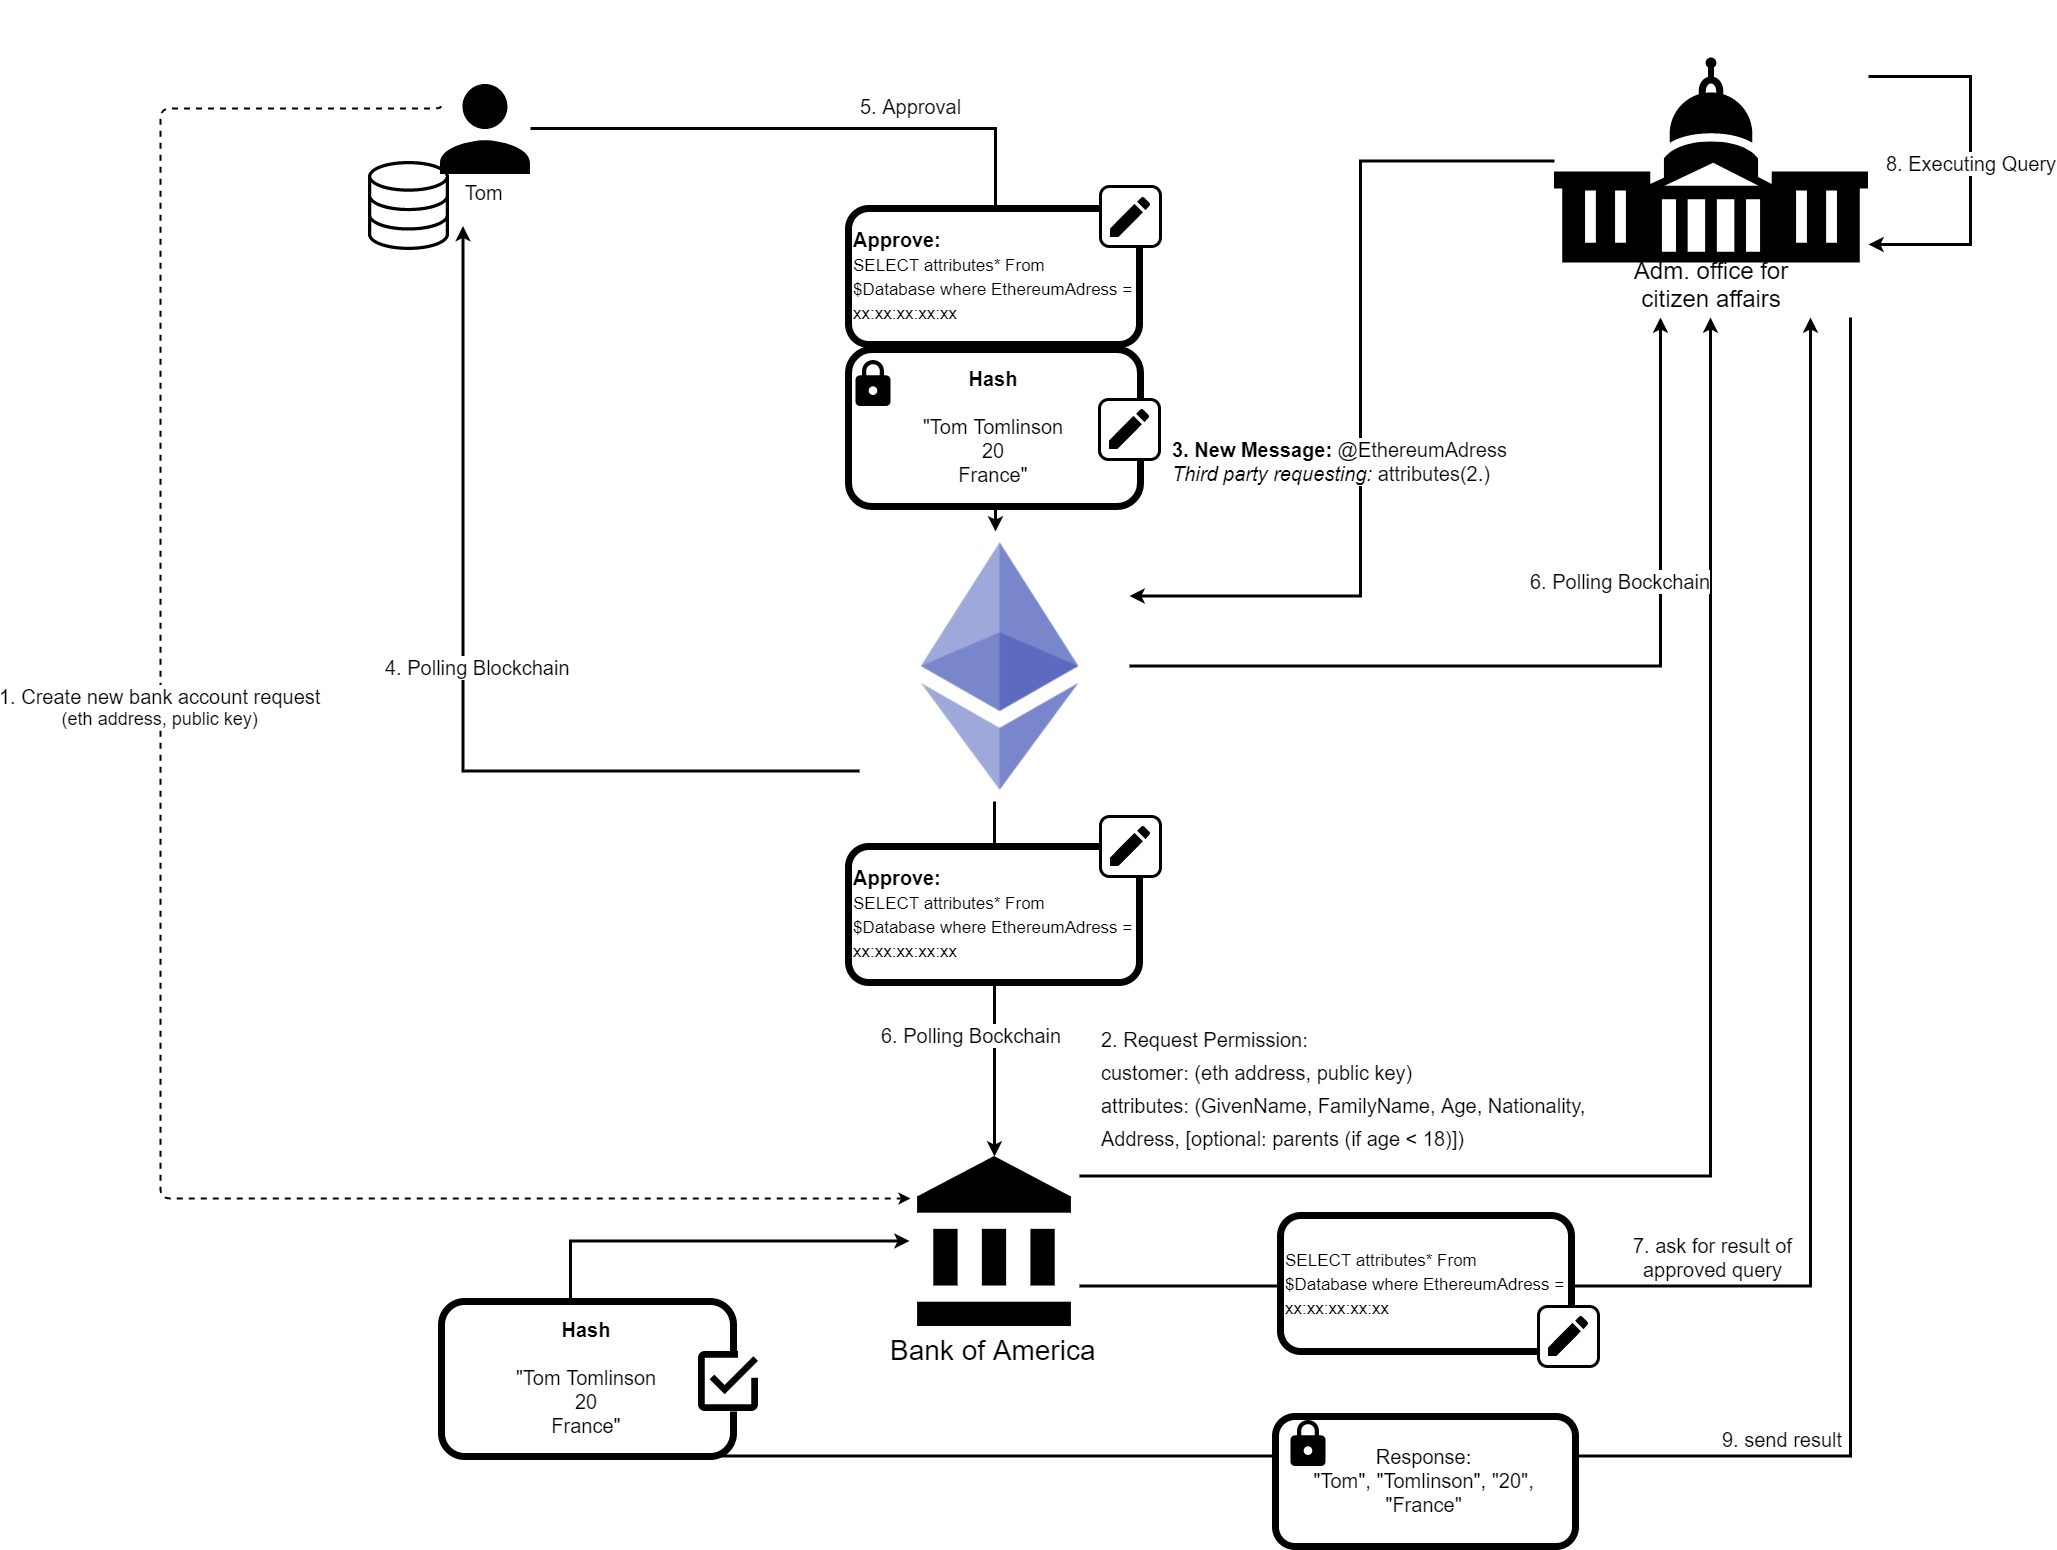
\includegraphics[width=\textwidth]{concept/permission_request_bank.png}

\subsection{Changing Attributes}

 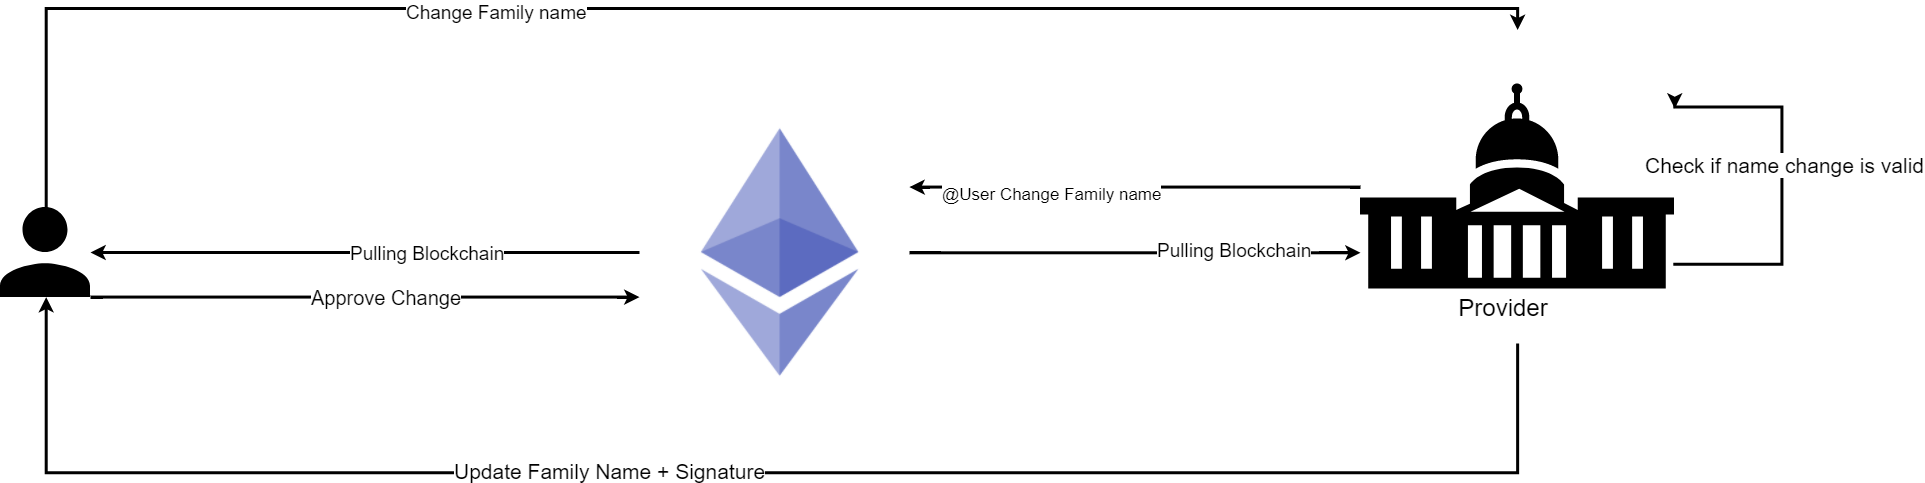
\includegraphics[width=\textwidth]{concept/change_attribute.png}

\subsection{Evaluation}

 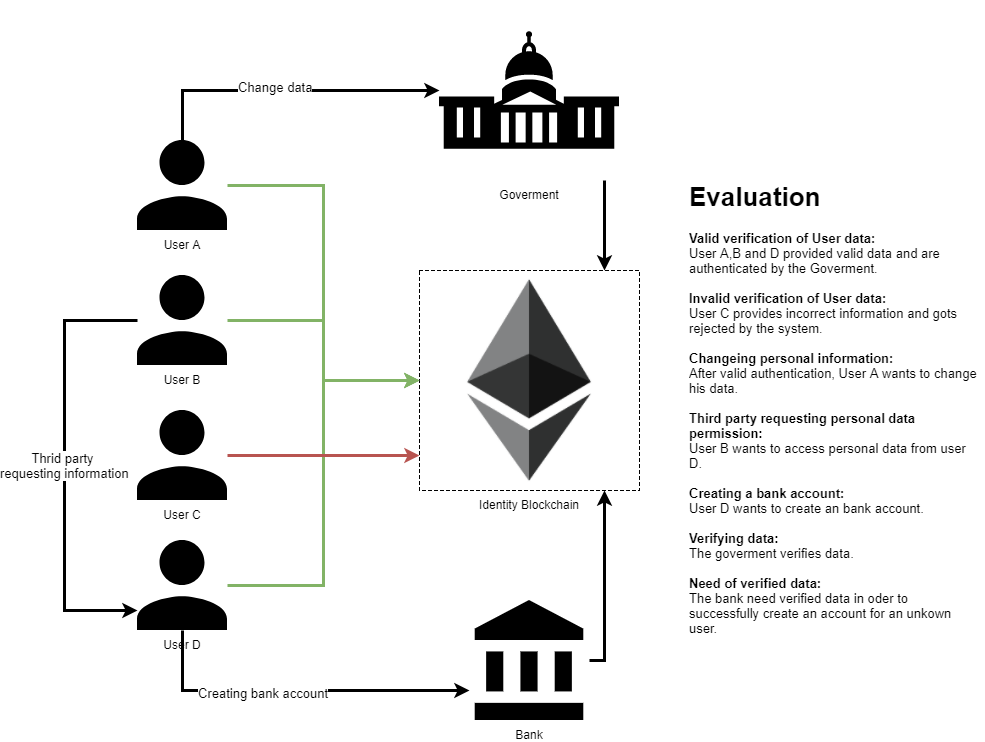
\includegraphics[width=\textwidth]{concept/evaluation.png}
 
\section{Use cases}

\subsection{Change a claim}
Lets have a user Bob Bobsen who has recently married Alice Alicson. Since Bob wants to change his family name to Bob Alicon this information needs to be updated in our system. To do so he sends a Update-Familiy-Name-Request with his new family name, to the corresponding identity provider, most likely the government. They on the other hand, can now verify this new claim by checking Bob's marriage contract. If all information match Bobs claims the identity provider publishes a Change-Family-Name-Claim transaction in the transaction blockchain to notify all third parties and other identity providers about the new claim of Bob's ID. 
Bob does then pull the blockchain, verifies the transaction code and approves the change by publishing his approval to the blockchain. The government permanently changes Bobs name in their database and sends the changes to Bob so that he can store the same changes in his local database. 
Each provider also holding bobs family name can then query the identity provider issued the name change again to pull the new name of Bob if Bob permitted this. (He could have done so by setting the "reuse" flag in the header of his signed query.)
The process described above will be processed in the same way when a third party requests a change of a claim. Bob on the other hand needs to explicitly approve this change. To model both transaction in the same way we hide the information who triggered the information change.
